\documentclass[12pt,english,portrait]{article}
\usepackage{babel}
\usepackage{html}
%\usepackage[colorlinks=true,urlcolor=blue,linkcolor=blue,menucolor=blue]{hyperref}
\usepackage{hyperref}
\usepackage{mdwlist}%allows tighter spacing when star on description*, enumerate* or itemize*
\usepackage{tabularx}
\usepackage{amsmath}
\usepackage{wrapfig}%allows text to wrap around figure
\usepackage{graphicx}
\usepackage{caption}
\usepackage{longtable}
\usepackage{multirow}
\usepackage{natbib}
\usepackage{booktabs} %makes nice tables
\usepackage{array}
\usepackage{fullpage}
% \usepackage{draftwatermark}%puts "draft" watermark on pages
\usepackage{verbatim}%enables multiline comments
\usepackage[backgroundcolor=white,textsize =small]{todonotes}% \todo{note} \todo[noline]{} \todo[inline]{} \missingfigure{} \listoftodos
\usepackage{listings} %provides syntax highlighting for code

% compressed itemized lists
\usepackage{mdwlist}
\let\stditemize\itemize
\let\endstditemize\enditemize
\let\itemize\undefined
\makecompactlist{itemize}{stditemize}
\let\stdenumerate\enumerate
\let\endstdenumerate\endenumerate
\let\enumerate\undefined
\makecompactlist{enumerate}{stdenumerate}


%\usepackage{biocon}
%\newplant{pavi2}{genus = Panicum, epithet=virgatum, author=L.}
%\newplant{misi}{genus = Miscanthus, epithet=sinensis, author=Andersson}
%\newplant{popul}{genus = Populus, author=L.}
%\newplant{salix}{genus = Salix, author=L.}
%\usepackage{xfrac}%provides \sfrac (slanted fractions)


\title{Data Entry Workflow\\for the \\Biofuel Ecophysiological Traits and Yields Database\\ \href{http://ebi-forecast.igb.uiuc.edu/bety/}{(BETYdb)}}
\author{Andy Tu, David LeBauer}

%\definecolor{darkgray}{gray}{0.25}

\begin{document}
\maketitle
\newpage

\listoffigures
\listoftables

\newpage

% header
\begin{figure}
  
\includegraphics[width=6.5in]{figures/db_header.png} 
\end{figure}

\section{Overview}
This is the userguide for entering data into the BETYdb database. 
The goal of this guide is to provide a consistent method of data entry that is transparent, reproducible, and well documented.
The steps here generally accomplish one of two goals. 
The first goal is to provide data in a consistent framework that is associated with the experimental methods, species, site, and other factors associated with the original study.
The second goal is to provide a record of all of the transformations, assumptions, and data extraction steps used to migrate data from the primary literature to the standardized framework of the database.
This second goal not only supports the scientific value of the data itself, it also simplifies the Quality Assurance process. 

\section{Mendeley: Managing citations}
Mendeley provides a central location for the collection, annotation, and tracking of the journal articles that we use.
Features of Mendeley that are useful to us include:
\begin{itemize*}
\item Collaborative annotation \& notes sharing, see section \ref{sec:annotate}
  \begin{itemize}
  \item text highlighter
  \item sticky notes for comments in the text
  \item notes field for text notes in the reference documentation
  \end{itemize} 
\item Read/unread \& favorites:  \\ Papers can be marked as as \textbf{read} or \textbf{unread}, and may be \textbf{stared}.
\item Groups: see section \ref{sec:groups}
\item Tagging
\end{itemize*}

\subsection{Creating a new group in Mendeley (Project Managers)} \label{sec:groups}

Each project has two groups, "projectname" and "projectname\_out" for the papers with data to be entered and the papers with data that has been entered. 
Papers in the \_out group may contain data for future entry, for example, traits that are not listed in \autoref{tab:traits}.

Each project manager may have one or more projects, each project should have one group.
Group names should refer to plant species, plant functional types, or other another project specific name. 
A list of current groups can be found in \autoref{tab:projects}. 
Please make sure that, at a minimum, Mike Dietze and David LeBauer are invited to join each project folder.


\begin{enumerate}
\item open Mendeley desktop 
\item \verb+Edit+ $\to$ \verb+Create Group+ or \texttt{Ctrl+Shift+M}
\item create group name following instructions above
\item enter group name 
\item set \verb+Privacy Settings+ $\to$ \verb+Private+
\item click \verb+Create Group+
\item click \verb+Edit+ $\to$ \verb+Settings+
\item check File \verb+Synchronization+ $\to$ \verb+Download attached files to group+
\end{enumerate}

\subsection{Adding and annotating papers (Project Managers)}\label{sec:annotate}

The 'tag' field associated with each paper can be used to further separate papers, for example by species, or the type of data ('trait', 'yield', 'photosynthesis') that they contain.  
When naming a group,  folders so that instructions for a technician would include the folder and the tag to look for, e.g.  "please enter data from projectx" or "please enter data from papers tagged y from project x".

To access the full text and pdf of papers from off campus, use the \href{http://www.cites.illinois.edu/vpn/download-install.html}{UIUC VPN} service.


If you are managing a Mendeley folder that undergraduates are actively entering data from, please plan to spend between 15 min and 1 hour per week maintaining it - enough to keep up with the work that the undergraduates are doing.

\subsubsection{Adding a reference to Mendeley}

\begin{itemize}
\item if the doi number is available (most articles since 2000)
\begin{enumerate}
\item select project folder
\item add entry manually
\item paste DOI number in \textit{DOI} field
\item select the search spyglass icon
\item drag and drop pdf onto the record. 
\end{enumerate}
\item If doi not available:
\begin{enumerate}
\item download the paper and save as  \verb+citation_key.pdf+
\item add using the \textit{Files} field
\item the citation key should be in \verb+authorYYYYabc+ where \verb+YYYY+ is the four digit year and \verb+abc+ is the acronym for the first three words excluding articles (the, a, an), prepositions (on, in, from, for, to, etc...), and the conjunctions (for, and, nor, but, or, yet, so) with less than three letters.
\end{enumerate}
\end{itemize}

\subsubsection{Annotating a Reference in Mendeley}
Each week, please identify and prepare papers that you would like to be entered next by completing the following steps:

\begin{enumerate}
\item Use the star label to identify the papers that you want the student to focus on next.

\begin{itemize}
\item Start by keeping a minimum of 2 and a maximum of 5 highlighted at once so that students can focus on the ones that you want. Students have been entering 1-3 papers per week, once we get closer to 3-5, the min/max should change.
\item Choose papers the papers that are the most data rich.
\end{itemize}

\item For each paper, use comment bubbles, notes field, and highlighter to indicate:

\begin{itemize}
\item name(s) of traits to be collected
\item methods:

\begin{itemize}
\item site name
\item location
\item number of replicates
\item statistics to collect
\item identify treatment(s) and control
\item indicate if study was conducted in greenhouse, pot, or growth chamber
\end{itemize}

\item data to collect

\begin{itemize}
\item identify figures number and the symbols to extract data from.
\item table number and columns with data to collect
\end{itemize}

\item covariates
\item management data (for yields)
\item units in 'to' and 'from' fields of \autoref{tab:traitconversion} used to convert data
\item esoteric information that other scientists or technicians might not catch and that are not otherwise recorded in the database
\item any data that may be useful at a later date but that can be skipped for now.
\end{itemize}

\end{enumerate}

\vspace{1em}
\noindent\textbf{Comment or Highlight}

\begin{itemize}
\item sample size
\item covariates (see \autoref{tab:covariates})
\item treatments
\item managements
\item other information entered into the database, e.g. experimental details
\end{itemize}

\subsection{Finding a citation in Mendeley}
 To find a citation in Mendeley, go to the project folder. 
Group folders and personel are listed in \autoref{tab:projects}. 
 By default, data entry technicians should enter data from papers which have been indicated by a yellow star and in the order that they were added to the list.
  Information and data to be collected from  paper can be found under the 'notes' tab and in highlighted sections of the paper. 

\begin{table}[bh]
  \caption{Current Projects}{List of current projects, PI's, Managers, and Technicians.}
  \label{tab:projects}
  \begin{tabularx}{\textwidth}{p{1in}lcccc}
    \hline 
    Folders & Project & PI & Manager & Technicians & Status\\
    \hline
    arctic & Arctic & M. Dietze & C. Davidson & M. Azimi& active\\
    prairie & Prairie & M. Dietze & X. Feng & {*}& active\\
    Poplar, Willow, Woody & Hardwood & M. Dietze & D. Wang & {*}N. Brady& active\\
    sugarcane & Sugarcane & F. Miguez & D. Jaiswal & F. Hussain& active\\
    syntheses&  synthesis papers& M. Dietze & D. LeBauer & {*}D. Bettinardi& complete\\
    face & FACE/NCEAS & M. Dietze & D. LeBauer & {*}Andy Tu& complete\\
    switchgrass & Switchgrass & M. Dietze & D. LeBauer & & inactive\\
    \hline
  \end{tabularx}
\end{table}


\section{Google Spreadsheets: Recording data transformations}\label{sec:googlespreadsheets}

Google Spreadsheets are used to keep a record of any data that is not entered directly from the original publication.

\begin{itemize}
\item any raw data that is not directly entered into the database but that is used to derive data or stats using equations in \autoref{tab:traitconversion} and \autoref{tab:statname}
\item any data extracted from figures, along with the figure number
\item any calculations that were made. These calculations should be included in the cells.
\end{itemize}

Each project has a google document spreadsheet with the title ''project\_data''.
In this spreadsheet, each reference should have a separate worksheet labeled with the citation key (\verb+authorYYYabc+ format).
Do not enter data into excel first, this is prone to errors and information such as equations may be lost when uploading or copy-pasting. 

\section{Redmine: Reporting errors, suggesting features}
\subsection{Reporting errors in Redmine }
\subsection{Suggesting features in Redmine}
 
\section{BETYdb: Entering new data through the web interface}

Before entering data, it is first necessary to (add and) select the citation that is the source of the data.
It is also necessary for each data point to be associated with a Site, Treatment, and Species.
Cultivar information is also required when available, but is only relevant for domesticated species.
Fields with an asterix (*) are required.

\subsection{Adding a Citation} 
Citation provides information regarding the source of the data. 
This section should allow us to locate and access the paper of interest.

A pdf copy of each paper should be available through Mendeley. 

\begin{enumerate}
\item Select one of the starred papers from your projects Mendeley folder.
\item The data to be entered should be specified in the notes associated with the paper in Mendeley
\item Identify (highlight or underline) the data (means and statistics) that you will enter
\item Enter citation information (\autoref{fig:citations_new})
  \begin{enumerate}
  \item \href{http://ebi-forecast.igb.uiuc.edu/bety/sites/new}{Data entery form} for a new site:  \verb+BETYdb+ $\rightarrow$ \verb+Citations+ $\rightarrow$\verb+new+  
  \item{Author} Input the first author's last name only 
  \item{Year} Input the year the paper was published, not submitted, reviewed,
    or anything else 
  \item For unknown information, input NA 
  \item{URL} web address of the article, preferably from publishers website
  \item{PDF} URL of the PDF of the article 
  \item{DOI} is the 'digital object identifier'. If DOI is available, PDF and URL are optional. This can be located in the article or in the article website. Use Ctrl+F 'DOI' to find it.  Some older articles do not have a DOI.
  \end{enumerate}
\end{enumerate}

\begin{figure}
  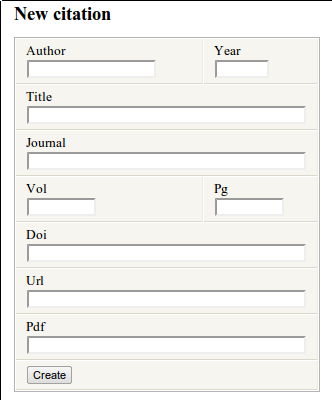
\includegraphics[width=2.5in]{figures/citations_new.png} 
  \caption{\href{http://ebi-forecast.igb.uiuc.edu/bety/citations/new}{Form for entering a new citation.}}
  \label{fig:citations_new}
\end{figure}

\subsection{Adding a Site}
 Each experiment is conducted at a unique site.
 In the context of BETY, the term 'site' refers to a specific location and it is common for many sites to be located within the same experimental station.
 By creating distinct records for multiple sites, it is possible to differentiate among independent studies.  

\begin{enumerate}
\item Before adding a site, search to make sure that site is not already entered in database.
\item search for the site given latitude and longitude
  \begin{itemize}
  \item if an institution name or city and state are given, try to locate the site on Google Maps
  \item if a site name is given, try to locate the site using a combination of Google and Google Maps
  \item if latitude and longitude are given in the paper, search by lat and lon, this will return all sites within $\pm1$ degree lat and long.
  \item if an existing site is plausibly the same site as the one mentioned in the paper, it will be necessary to check other papers linked to the existing site. 
    \begin{itemize}
    \item use the same site if the previous study uses the \emph{exact same location} and experimental setup. 
    \item create a new site if the study was conducted in a different fields (i.e., not the exact same location).
    \item create a new site if one study was conducted in a greenhouse and another in a field.
    \item do not use distinct sites for seed source in a common garden experiment (see 'When not to enter a new site' below) 
    \end{itemize}  
  \end{itemize} 
\item to use an existing site, click 'edit' for the site, and then select current citation under 'add citation relatinships' 
\item if site does not exist, add a new site.
\end{enumerate}

 \todo[inline]{\textbf{When not to enter a new site:} When plants (or seeds) are collected from multiple locations and then grown in the same location, this is called a 'common garden experiment'. In this case, the location of the study is included as site information. Information about the seed source can be entered as a distinct cultivar.}



\begin{description}
\item[Site name*] Site identifier, sufficient to uniquely identify the site within the paper
\item[City] Nearest city
\item[State] State, if site is in US
\item[Country*]
\item[Longitude*]
\item[Latitude*] Latitude and Longitude must be in decimal form. To convert minute-second to decimal degrees, see the equation in \autoref{tab:traitconversion}. 
\item[Greenhouse*] set Greenhouse = TRUE if plants were grown in a greenhouse, growth chamber, or pots. If a 'warming chamber' or 'greenhouse' is used as the experimental manipulation, but is not used in the control treatments, Greenhouse = FALSE.
\item[Soil] Soil class is entered as a categorical variable that describes the texture. If percent clay, sand, and silt are given, \autoref{fig:soiltexture} can be used to look up the class.
\item[SOM] Soil organic matter (\% by weight)  
\item[MAT]  Mean Annual Temperature ($^o$C)
\item[MAP]  Mean Annual Precipitation (mm)
\item[MASL]    Elevation (meters above sea level, m)   
\item[Notes] site details not included above
\item[Soilnotes] soil details not included above  
\item[Rooting Zone Depth] Depth of rooting zones in meters      
\item[Depth to Water Table]  Depth to water table in meters
\end{description}


\begin{figure}
  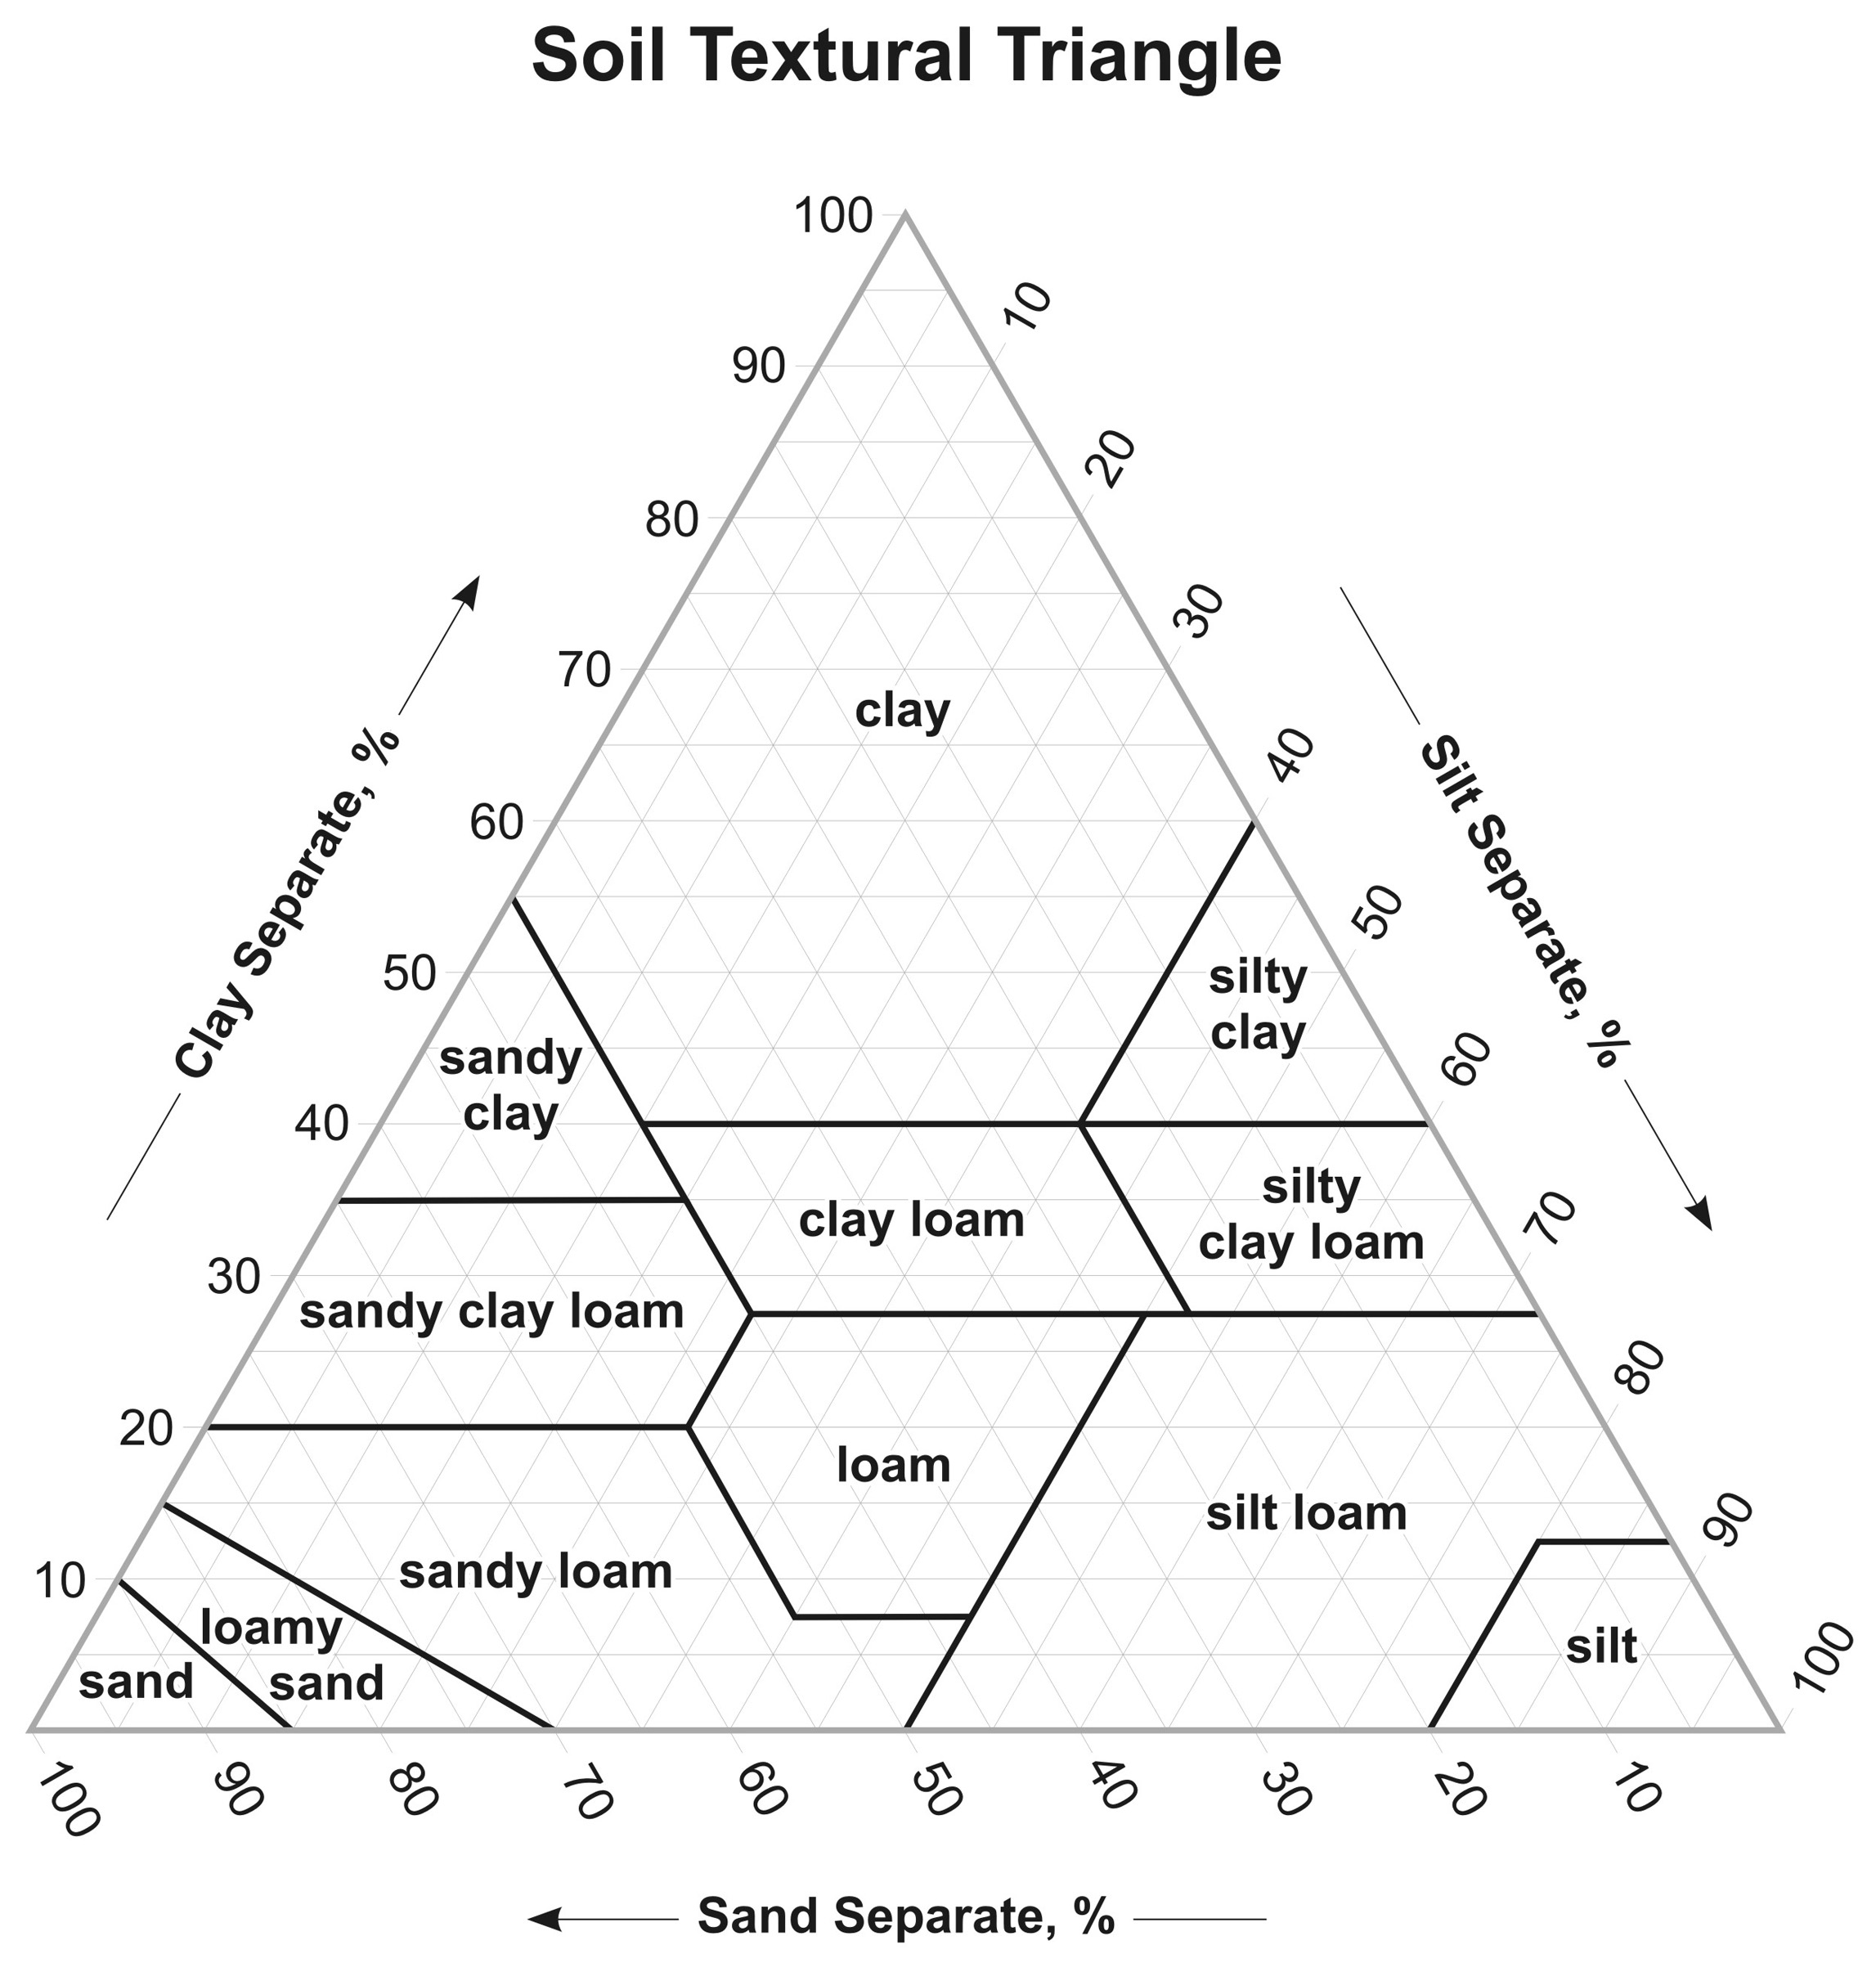
\includegraphics[width=4in]{figures/soiltexture.png} 
  \caption{\href{http://soils.usda.gov/education/resources/lessons/texture/}{USDA soil classification.} }
  \label{fig:soiltexture}
\end{figure}


\begin{figure}
  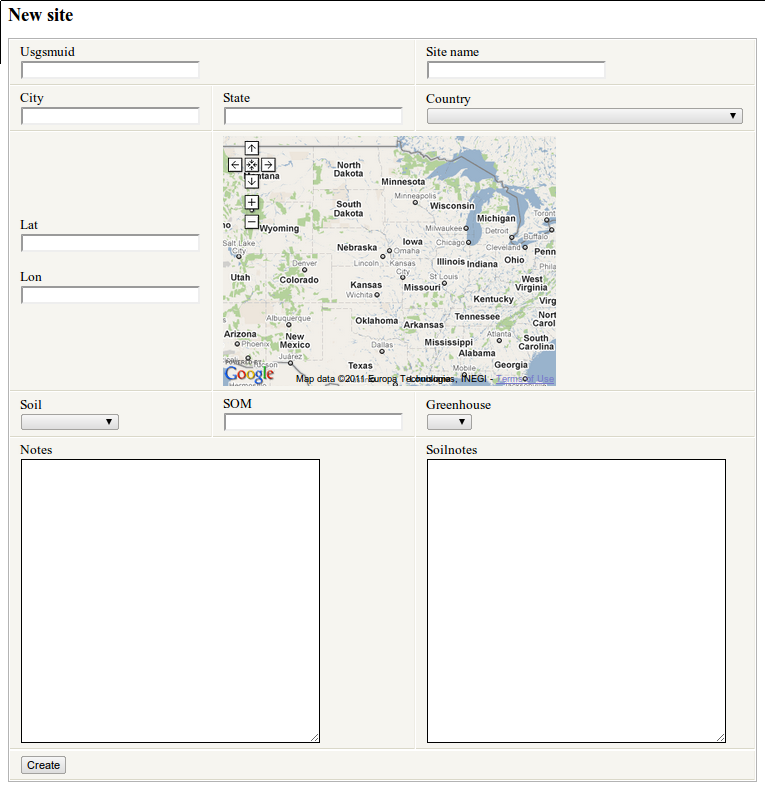
\includegraphics[width=4in]{figures/sites_new.png} 
  \caption{\href{http://ebi-forecast.igb.uiuc.edu/bety/sites/new}{Form for entering a new site.} }
  \label{fig:sites_new}
\end{figure}

\subsubsection{Site Location}


 If latitude and longitude coordinates not available, it is often possible to determine the site location based on the site name, city, and other information.
 One way to do this would be to look up a location name in \href{http://maps.google.com}{google maps} and then locate it on the embedded map.
 Google Maps can provide decimal degrees if the LatLng feature is enabled, which can be done \href{http://maps.google.com/maps?showlabs=1}{here}.
 Google Earth can be particularly useful in locating sites, along with their coordinates and elevation.
 Alternatively, the site website or address might be found through an internet search (e.g. Google).

 Use \autoref{tab:siteloc} to determine the number of significant digits to indicate the level of precision with which a study location is known.

\begin{table}
\caption{Appropriate precision for site latitude and longitude}
\label{tab:siteloc}
\begin{tabular}{rl}
\hline
                  & decimal degree\\
 location detail  &   accuracy  \\
\hline
 city             &                      0.1  \\
 mile             &                     0.01  \\
 acre             &                    0.001  \\
 10 meters        &                   0.0001  \\
\hline
\end{tabular}
\end{table}


\subsection{Adding a Treatment}\label{sec:addtreatment}
 Treatments provide a description of a study's treatments. 
 Any specific information such as rate of fertilizer application should be recorded in the managements table (section \autoref{sec:addmanagement}).
 In general, managements are recorded when Yield data is collected, but not when only Trait data are collected.

 \todo[inline]{\textbf{When not to use treatment:} predictor variables that are not based on distinct managements, or that are distinguished by information already contained in the trait table (e.g. site, cultivar, date fields) should not be given distinct treatments. For example, a study that compares two different species, cultivars, or genotypes can be assigned the same control treatment; these categories will be distinguished by the species or cultivar field. Another example is when the observation is made at two sites: the site field will include this information.}   

 A treatment name is used as a categorical (rather than continuous) variable: it should be easy to find the treatment in the paper based on the name in the database.
 The treatment name does not have to indicate the level of treatment used in a particular treatment - this information will be included in management table.
 
 It is essential that a control group be identified with each study.
 If there is no experimental manipulation, there is only one treatment.
 In this case, the treatment should be named 'observational' and listed as control.

 To determine the control when it is not explicitly stated, first determine if one of the treatments is most like a background condition or how a system would be in its non-experimental state.
 In the case of crops, this could be how a farmer would be most likely to treat a crop.

\begin{figure}[hb]
  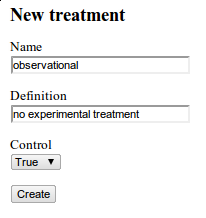
\includegraphics[width=2in]{figures/treatment_new.png} 
  \caption{\href{http://ebi-forecast.igb.uiuc.edu/bety/treatments/new}{Form for entering a new treatment.} }
  \label{fig:treatment_new}
\end{figure}


\begin{figure}[hb]
  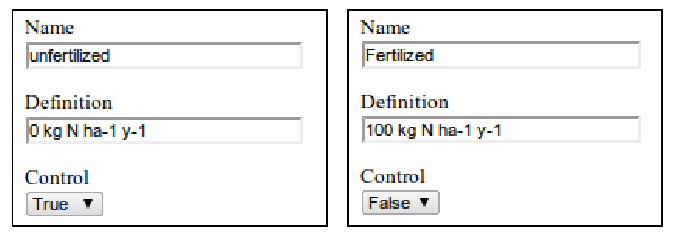
\includegraphics[width=3in]{figures/treatment_examples.pdf} 
  \caption{Example treatment form with control and experimental information}{Example of data entered into the treatment form for a control (left) and treatment (right)}
  \label{fig:treatment_examples}
\end{figure}


\begin{description}
\item[Name] indicates type of treatment; it should be easy for anyone with the original paper to be able to identify the treatment from its name.
\item[Control] make sure to indicate if the treatment is the study 'control' by selecting true or false 
\item[Definition] indicates the specifics of the treatment. 
It is useful for identification purposes to use a quantified description of the treatment even though this information can only be used for analysis when entered as a management. 
\end{description}

\subsection{Adding a Management}\label{sec:addmanagement}

 Managements refers to something that occurs at a specific time and has a quantity; 
 Managements include actions that are done to a plant or ecosystem, for example the planting density or rate of fertilization.
 Managements are distinct from Treatments in that a Treatment is used to categorically identify an experimental treatment, whereas a management is used to describe what has been done.


Managements are the way a treatment becomes quantified.
Each treatment is often associated with multiple managements. 
The combination of managements associated with a particular treatment will distinguish it from other treatments.
The management types that can be entered into BETY are described in \autoref{tab:mgmttype}. 

Each management may be associated with one or more treatments. For example, in a fertilization experiment, planting, irrigation, and herbicide managements would be applied to all plots but the fertilization will be specific to a treatment.
For a multi-year experiment, there may be multiple entries for the same type of management, reflecting, for example, repeated applications of herbicide or fertilizer, for example see \autoref{fig:trtmgmt}.

\emph{note:}  At present, managements are recorded for Yields but not for Traits, unless specifically required by the data or project manager.

\begin{figure}
\caption{Form for entering and editing relationships between treatments and managments}
\label{fig:trtmgmt}
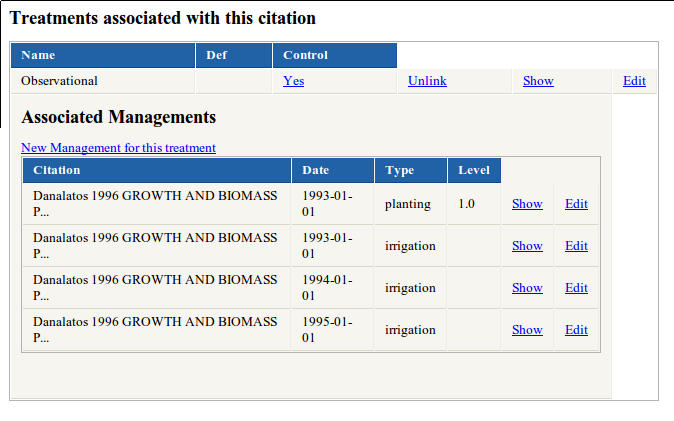
\includegraphics[width=5in]{figures/treatments_managements.png}
\end{figure}

\begin{figure}
  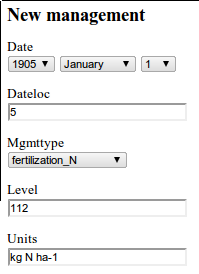
\includegraphics[width=2in]{figures/management_new.png} 
  \caption{Form for entering new managment}{Form for entering management data with example data. This management denotes a nitrogen fertilization rate of 112.0 kg N ha-1.}
\label{fig:management_new}
\end{figure}
 
To associate a management with multiple treatments, first create the management, then edit the management and add treatment relationships. 

 \begin{description}
 \item[mgmttype] the name of the management being used. A list of standardized management types can be found in \autoref{tab:mgmttype}.
 \item[Level] a quantification of mgmttype. 
 \item[units] refers to the units of the level. Units should be converted to those in \autoref{tab:mgmttype}.
 \item[dateloc] date level of confidence, explained in \autoref{sec:traits} and defined in \autoref{tab:traits}.
\end{description}


\begin{table}[hb]
  \caption{Managements}{This is a list of  managements to enter, with the most common management types in \textbf{bold}. It is more important to have management records for Yields than for traits. For greenhouse experiments, it is not necessary to include informaton on fertilizaton, lighting, or greenhouse temperature.}
  \label{tab:mgmttype}
  \begin{tabularx}{\linewidth}{rcp{1.5in}p{1.5in}}
    \hline
    \textbf{Management Type} & Units & Definition & notes\\ \hline
    burned & & aboveground biomass burned & \\
    CO2\_fumigation&ppm & & \\
    \textbf{fertilization\_\textit{X}} & kg \textit{X} ha$^{-1}$ & fertilization rate, element \textit{X} &  \\
    fungicide & kg ha$^{-1}$ & &add type of fungicide to notes \\
    grazed& years & livestock grazing &pre-experiment land use\\
    \textbf{harvest} & & & no units, just date, equivalent to coppice, aboveground biomass removal \\
    \textbf{herbicide} & kg ha$^{-1}$ & &add type of herbicide to notes: glyphosate, atrazine, many others \\
    \textbf{irrigation} &cm & & convert volume / area to depth as required\\
    light &W m$^{-2}$ & & \\ 
    O3\_fumigation&ppm & & \\
    pesticide & kg ha$^{-1}$ & &add type of pesticide to notes \\
    \textbf{planting}  & plants m$^{-2}$ & &convert row spacing to planting density if possible \\
    \textbf{seeding}   & kg seeds ha$^{-1}$ & &\\
    tillage & & &no units, maybe depth; \emph{tillage} is equivlent to \emph{cultivate}\\
    \hline
  \end{tabularx}
\end{table}


\subsection{Adding a Trait}\label{sec:traits}

 In general, a 'trait' is a phenotype; a characteristic that the plant exhibits.
 The traits that we are primariliy interested in collecting data for are listed in \autoref{tab:traits}. 

 \begin{figure}[htb]
   \centering
   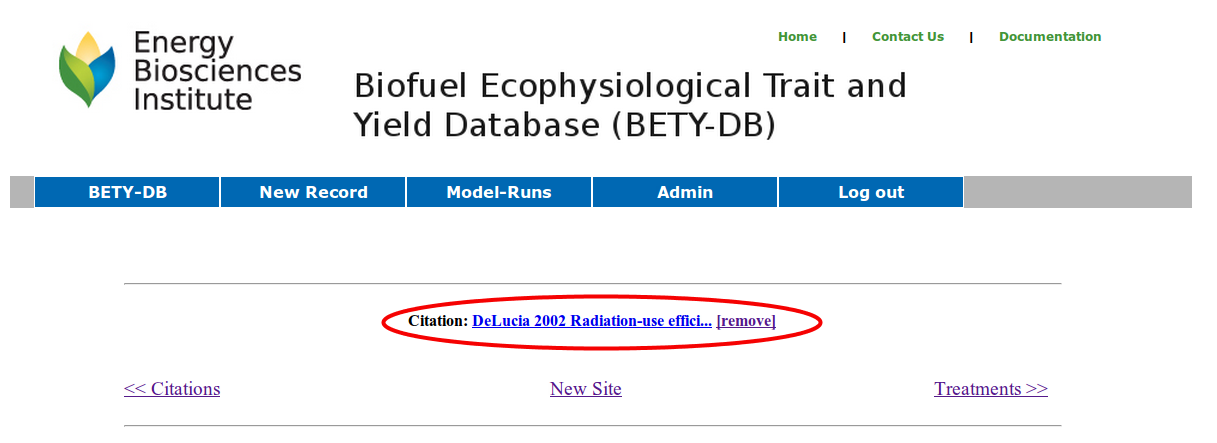
\includegraphics[width = 4in]{selectedcitation.png}
   \caption{When entering data, the citation is identified at the top of the page.}
   \label{fig:selected.citation}
 \end{figure}

 Before adding trait data, it is necessary to have the citation, treatments, and site information already entered.
 If the correct citation is not identified at the top of the page \autoref{fig:selected.citation}.
 To add a new Trait, go to the \href{http:ebi-forecast.igb.uiuc.edu/bety/traits/new}{new trait} page: \verb+Trait+ $\to$ \verb+new+.

 Presently, we are also using the Trait table record ecosystem level measurements other than Yield.
 Such ecosystem level measurements can include leaf area index or net primary productivity, but are only collected when required for a particular project. 

 \autoref{fig:traits_new} shows the web form for entering new trait data, and \autoref{tab:traits} provides a list of the traits that we are interested in collecting.

Most of the fields in the Traits table are also used in the Yields table.
Here is a list of the fields with a brief description, followed by more thorough explanations:

\begin{description}
\item[Species*] Search for species in the database using the search box; if species is not found, see \hyperref[sec:addspecies]{Section \ref*{sec:addspecies} Adding a Species} 
\item[Cultivar] primarily used for crops; If the cultivar being used is not found in drop-down box, see hyperref[sec:addcultivar]{Section \ref*{sec:addcultivar}: Adding a Cultivar}.
\item[DateLOC] Date Level of confidence. See \autoref{tab:dateloc} for values.
\item[Mean*] mean is in units of tons per hectare per year (t/ha) 
\item[Stat name] is name of the statistical method used (usually one of SE, SD, MSE, CI, LSD, HSD, MSD). See \hyperref[sec:stats]{section \ref*{sec:stats}} for more details.
\item[Statistic] is the value of the statistic associated with Stat name.
\item[N] Always record N if provided. N is the number of experimental replicates, often referred to as the sample size; N represents the number of independent units within each treatment: in a field setting, this is often the number of plots in each treatment, but in a greenhouse, growth chamber, or pot-study this may be the number of chambers, pots, or individual plants. Sometimes this value is not clearly stated.   

\end{description}

\subsubsection{dateloc}

 The date level of confidence (DateLOC) provides an indication of how accurately the date associated with the trait or yield observation is known.
 \autoref{tab:dateloc} provides the values that should be entered in this field. 
  If the event occurred at a level of precision not defined by an integer in this table, use fractions. 
 For example, we commonly use 5.5 to indicate a one week level of precision. 
 If the exact year is not known, but the time of year is, use 91 to 97, with the second digit to indicate the information known within the year.

\begin{table}
  \caption{Date level of confidence (DateLOC) Field}{Numbering convention for the DateLOC (Date level of confidence) field, used in managements, traits, and yields table. }
  \label{tab:dateloc}
  \begin{tabular}{rl}
    \hline
    Dateloc &  Definition\\
    \hline 
    9 & no data \\
    8 & year \\
    7 & season \\
    6 & month \\
    5 & day \\
    4 & time of day i.e. morning, afternoon \\
    3 & hour \\
    2 & minute \\
    1 & second \\
    95 & unknown year, known day \\
    96 & unknown year, known month \\
    ... etc& \\ \hline
  \end{tabular}
\end{table}

\subsubsection{Statistics}\label{sec:stats}

Our goal is to record statistics that can be used to estimate standard deviation or standard error.
Many different methods can be used to summarize data, and this is reflected in the diversity of statistics that are reported. 
 An overview of these methods is given in \autoref{tab:statname} and a description below.

 Where available, direct estimates of variance are preferred, including Standard Error (SE), sample Standard Deviation (SD), or Mean Squared Error (MSE).
 SE is usually presented in the format of $\text{mean} (\pm \text{SE})$.
 MSE is usually presented in a table.
 When extracting SE or SD from a figure, measure from the mean to the upper or lower bound.
 This is different than confindence intervals and range statistics (described below), for which the entire range is collected. 
  
 If MSE, SD, or SE are not provided, it is possible that LSD, MSD, HSD, or CI will be provided. 
 These are range statistics and the most frequently found range statistics include a Confidence Interval (95\%CI), Fisher's Least Significant Difference (LSD), Tukey's Honestly Significant Difference (HSD), and Minimum Significant Difference (MSD).
 Fundamentally, these methods calculate a range that indicates whether two means are diffent or not, and this range uses different approaches to penalize multiple comparisons.
 The important point is that these are ranges and that we record the entire range.

 Another type of statistic is a ``test statistic''; most frequently there will be an F-value that can be useful, but this should not be recorded if MSE is available.
 Only if there is no other information available, record the P-value.


\begin{table}
  \caption{List of statistical summaries}{List of the statistics that can be  entered into the statname field of traits and yields tables. Please see David (or Mike) if you have questions about statistics that do not appear in this list. If you have P, or LSD in a study with $n\neq b$ (e.g. not a RCBD, see \autoref{tab:statconversions}), please convert these values prior to entering the data, and add a note that stat was transformed to the table. Note: These are listed in order of preference, e.g., if SD, SE, or MSE are provided then use these values}
  \label{tab:statname}
  \begin{tabular}{lllp{2in}}
    \hline
    statname & name & definition &notes \\ \hline
    \textbf{SD}   & Standard Deviation, $s$ &$\sqrt{\frac{1}{N} \sum{(x_i - \bar{x})^2}}$ & $\bar{x}$ is the mean \\
    \textbf{SE}   & Standard Error& $\frac{s}{\sqrt{n}}$& \\
    \textbf{MSE} &Mean Squared Error &  & like SD, but with multiple treatments. in R: $\frac{mean(aov(y~x)\$residuals^2}{aov(y~x)\$df}$ \\
    \textbf{95\%CI} &95\% Confidence Interval & $t_{1-^{\alpha}/_2,n}*s$ & measure the 95\% CI from the mean, this is actually $^1/_2$ of the CI \\
    \textbf{LSD} & Least Significant Difference &$t_{1-\frac{\alpha}{2},n}\sqrt{2\text{MSE}/b}$ &$b$ is the number of blocks (Rosenberg 2004)\\%\cite{rosenberg2004map}\\
    \textbf{MSD} & Minimum Significant Difference & & \\
    \hline
  \end{tabular}
\end{table}


\begin{figure}

\includegraphics[width=3in]{figures/traits_new.png} 
\caption{Form used to enter a new trait.}
\label{fig:traits_new}
\end{figure}

\begin{table}
  \begin{tabular}{p{1.7in}p{1.7in}p{1.25in}p{2in}}
    \hline    
    Variable  & units & median (90\%CI) or range & definition \\
    \hline
    \href{http://ebi-forecast.igb.uiuc.edu/bety/variables/4}{Vcmax} &$\mu$mol CO$_2$ m$^{2}$ s$^{-1}$ &$44 (12, 125)$ & maximum rubisco carboxylation capacity\\
    \href{http://ebi-forecast.igb.uiuc.edu/bety/variables/15}{SLA}  & m$^2$ kg$^{-1}$ &$15(4,27)$ 
    & Specific Leaf Area area of leaf per unit mass of leaf \\
    \href{http://ebi-forecast.igb.uiuc.edu/bety/variables/254}{LMA} &   kg m$^{-2}$ & $0.09 (0.03, 0.33)$ 
    & Leaf Mass Area (LMA = SLM = 1/SLA) mass of leaf per unit area of leaf  \\
    \href{http://ebi-forecast.igb.uiuc.edu/bety/variables/10}{leafN}  & \% & $2.2(0.8, 17)$  
    & leaf percent nitrogen\\ 
    \href{http://ebi-forecast.igb.uiuc.edu/bety/variables/31}{c2n leaf}  &  leaf C:N ratio &$39(21,79)$ &  use only if leafN not provided \\
    \href{http://ebi-forecast.igb.uiuc.edu/bety/variables/40}{leaf turnover rate} & 1/year&$0.28(0.03,1.0) $ & \\
    \href{http://ebi-forecast.igb.uiuc.edu/bety/variables/5}{Jmax} & 	$\mu$mol photons m$^{-2}$ s$^{-1}$& $121(30, 262)$& maximum rate of electron transport \\ 
    \href{http://ebi-forecast.igb.uiuc.edu/bety/variables/26}{stomatal slope}  &  &$9(1, 20)$ & \\
    \href{http://ebi-forecast.igb.uiuc.edu/bety/variables/9}{GS} &  & & stomatal conductance (= gs$_{\textrm{max}}$ \\ 
    \href{http://ebi-forecast.igb.uiuc.edu/bety/variables/21}{q}{*} & &0.2--5 & ratio of fine root to leaf biomass\\
    \hspace{0.5em}*\emph{grasses}:  &  ratio of root:leaf $ =$ below~:~above ground biomass \\
    \hspace{1em} aboveground biomass  &  g m$^{-2}$ \emph{or} g plant$^{-1}$ & &\\
    \hspace{1em} root biomass  & g m$^{-2}$ \emph{or} g plant$^{-1}$ & & \\
    \hspace{0.5em}*\emph{trees}:  &  ratio of fine root:leaf biomass  \\
    \hspace{1em} leaf biomass & g m$^{-2}$  \emph{or} g plant$^{-1}$& & \\ 
    \hspace{1em} fine root ($<$2mm) biomass  & g m$^{-2}$ \emph{or} g plant$^{-1}$ & & \\
    \href{http://ebi-forecast.igb.uiuc.edu/bety/variables/41}{root turnover rate}  &1/year &0.1--10 & rate of fine root loss (temperature dependent) year$^{-1}$ \\
    \href{http://ebi-forecast.igb.uiuc.edu/bety/variables/22}{leaf width}  & mm &22(5,102) &  \\
    \href{http://ebi-forecast.igb.uiuc.edu/bety/variables/27}{growth respiration factor}  &\% & 0--1 & Proportion of daily carbon gain lost to growth respiration  \\
    \href{http://ebi-forecast.igb.uiuc.edu/bety/variables/7}{R$_{\textrm{dark}}$} & & $\mu$mol CO$_2$ m$^{-2}$ s$^{-1}$ & dark respiration\\
    \href{http://ebi-forecast.igb.uiuc.edu/bety/variables/39}{quantum efficiency} & \% & 0--1& efficiency of light conversion to carbon fixation, see Farqhuar model,  \\
    \href{http://ebi-forecast.igb.uiuc.edu/bety/variables/29}{dark resp factor}  &  \% & 0--1&converts Vm to leaf respiration \\
    \href{http://ebi-forecast.igb.uiuc.edu/bety/variables/44}{seedling mortality} &  \% & 0--1&proportion of seedlings that die \\
    \href{http://ebi-forecast.igb.uiuc.edu/bety/variables/192}{r fract}  & \% & 0--1&fraction of storage to seed reproduction \\
    \href{http://ebi-forecast.igb.uiuc.edu/bety/variables/244}{root respiration rate}{*} &CO$_2$ kg$^{-1}$ fine roots s$^{-1}$ &1--100 & rate of fine root respiration at reference soil temperature \\
    \href{http://ebi-forecast.igb.uiuc.edu/bety/variables/49}{f labile}  & \% & 0--1&fraction of litter that is goes into the labile carbon pool  \\
    \href{http://ebi-forecast.igb.uiuc.edu/bety/variables/45}{water conductance}  &  & & \\
    \hline
  \end{tabular}
  \caption[Table of traits]{Table of traits to be entered. Notes: \textbf{\texttt{q}}: if only \texttt{q} is available, record this value, otherwise record either total root and total aboveground (for grasses) or fine root and leaf biomass (for trees) data when these are available.
 For calculating \texttt{q}, units may be per area or per plant, but must be the same for both the aboveground/leaf and belowground/fine root components.
 \texttt{q} is calculated from fine root and leaf biomass that are associated with the same \texttt{treatment}, \texttt{date}, \texttt{species}, \emph{and} \texttt{site}.
 \textbf{\texttt{root\_respiration\_rate}}: represents the total root respiration, \textbf{\texttt{root\_respiration\_factor}} is an ED parameter that represents the maintenance respiration, for which little (if any) data is available. Only if root \emph{maintenance} respiration data is found, the \texttt{root\_respiration\_factor} variable should be used.}
  \label{tab:traits}
\end{table}



\subsection{Adding a Yield}

The protocol for entering yield data is identical to entering data for a trait, with a few exceptions:

\begin{enumerate}
\item There are no covariates associated with yield data 
\item Yield data is always the dry harvestable biomass; if necessary, moisture content can be added as a trait
\end{enumerate}

\subsection{Adding a Covariate} 

 Covariates are required for many of the traits.
 Covariates generally indicate the environmental conditions under which a measurement was made.
 Without covariate information, the trait data will have limited value.

 A complete list of required covariates can be found in \autoref{tab:covariates}. 
 For all respiration rates and photosynthetic parameters, temperature is recorded as a covariate. 
 Soil moisture, humidity, and other such variables that were measured at the time of the measurement that may be required in order to standardize across studies.

 When root data is recorded, the root size class needs to be entered as a covariate.
 The term 'fine root' often refers to the <2mm size class, and in this case, the covariate \verb+root_maximum_diameter+ would be set to $2$. 
 If the size class is a range, then the \verb+root_minimum_diameter+ can also be used.
 
 To add a new covariate, go to the \href{http:ebi-forecast.igb.uiuc.edu/bety/covariates/new}{new covariate} page: \verb+Covariate+ $\to$ \verb+new+.
 
\begin{table}
  \begin{tabular}{p{2in}p{2in}p{2in}}
    \hline
    variable &required covariates& optional covariates \\ \hline
    Vcmax&irradiance and temperature (leaf or air)  & \\
    any leaf measurement & & canopy height \\
    root\_respiration\_rate& temperature (root or soil)   & soil moisture \\
    root\_respiration\_rate&root\_diameter\_max & root size class (usually $<2mm$) \\
    any respiration &temperature & \\
    root biomass & & min size cutoff, max size cutoff\\
    root, soil & depth (cm)  & used for max and min depths of soil, if only one value, assume min depth = 0; negative values indicate above ground\\
    gs (stomatal conductance)&A$_{max}$ & \dag see notes in caption\\
    stomatal\_slope (m) & humidity, temperature &?specific humidity? assume leaf T =  air T? \\ 

  \end{tabular}
  \caption{Traits with required covariates}{A list of traits and the covariates that must be recorded along with the trait value in order to be converted to a constant scale from across studies. \emph{notes:} $\dag$ stomatal conductance (gs) is only useful when reported in conjunction with other photosynthetic data, such as A$_{max}$. Specifically, if we have Amax and gs, then estimation of Vcmax only covaries with \texttt{dark\_respiration\_factor} and atmospheric CO2 concentration.  We also now have information to help constrain \texttt{stomatal\_slope}. If we have \texttt{Amax} but not \texttt{gs}, then our estimate of \texttt{Vcmax} will covary with: \texttt{dark\_respiration\_factor}, CO$_2$, \texttt{stomatal\_slope}, \texttt{cuticular\_conductance}, and vapor-pressure deficit (\texttt{VPD}) (which is more difficult to estimate than CO$_2$, but still possible given lat, lon, and date). 
 Most important, there will be a strong covariance between \texttt{Vcmax} and \texttt{stomatal\_slope}.}
  \label{tab:covariates}
\end{table}

\subsubsection{Extracting information from tables and graphs}
\begin{enumerate}
\item identify the data that is associated with each treatment\\

  \textit{note:}\small{if the experiment has many factors, the paper may not report the mean and statistics for each treatment. Often, the reported data will be reflect the results of more than one treatment, for example if there was no effect of the treatement on the quantity of interest. In some cases it will be possible to calculate the values for each treatment, e.g. if there are $n-1$ values and $n$ treatments. If this is not the case, the treatment names and definitions should be changed to indicate that data reflect the results of more than one experimental treatments}
\item enter the mean value of the trait
\item enter the \verb+statname+, \verb+stat+, and number of replicates, \verb+n+ associated with the mean 
  \begin{itemize}
  \item \verb+stat+ is the value of the \verb+statname+ (i.e. \verb+statname+ might be 'standard
    deviation' (SD) and the \verb+stat+ is the numerical value of the statistic) 
  \item always measure size of error bar from the mean to the end of an error bar. This is
    the value when presented as $X\pm SE$ or $X(SE)$ and may be found in a table or
    on a graph. 
  \item sometimes CI and LSD are presented as the entire range from the lower to the upper end of the confidence interval. In this case, take 1/2 of the interva representing the distance from the mean to the upper or lower bound 
  \end{itemize}
\end{enumerate}

\subsubsection{Extracting Data From a Figure using R}

To extract data from a jpg file in R using the digitize package:

\begin{enumerate}
\item save image as a \verb+*.jpg+ file
\item open R
\item change the directory that R is using to the one where the image is
\item use R code below to extract data, display it, and save it in a \verb+csv+ file steps below  
\item upload csv to the project file in google spreadsheet, or open as excel/openoffice and copy/paste to google spreadsheet 
\end{enumerate}

\begin{verbatim}
library('digitize')
calpts <- ReadAndCal('authorYYYabc_fixX.jpg') 
   ## click on xaxis min (x1), xaxis max (x2), 
   ## yaxis min(y1), yaxis max (y2)
pts <- DigitData(col='red',type='p',n=8)
   ## set n = to the number of points to collect 
data <- Calibrate(pts, calpts, x1, x2, y1, y2)
   ## x1, x2, y1, and y2 are the min and max of the x and y axes, respectively.
print(data)
write.csv(data, 'authorYYYYabc_figX.csv')
\end{verbatim}

\subsubsection{Extracting Data From a Figure using GetData}
\begin{enumerate}
\item Open pdf in Adobe Reader.
\item Zoom in on the figure
\item Choose \verb+Tools+ $\to$ \verb+Select and Zoom+
\item Open Paint
\item Paste Picture
\item Save as authorYYYYabc\_figX.jpg
\item Open Get Data
\item \verb+File+ $\to$ \verb+open+ open figure
\item select button with two arrows (fourth from left)
\item follow instructions to select x min, x max, y min and y max. If the x-axis has a categorical variable, it does not matter what values you use for x min and x max.
\item make sure to set the correct values for the max and min of each axis, and indicate if the axis is log-scaled
\item select the target button (seven from left)
\item click over center of desired data points and error bars
\item copy data to google spreadsheet (see Section \ref{sec:googlespreadsheets}
\item calculate SE as the distance between the error bar upper bound and the mean (absolute value of difference between the two points) 
\end{enumerate}

\subsection{Adding a Yield} 

 To add a new Yield, go to the \href{http:ebi-forecast.igb.uiuc.edu/bety/yields/new}{new yield} page: \verb+Yield+ $\to$ \verb+new+.
 Yield is equivalent to aboveground biomass on a per-area basis, and has units of Mg ha$^{-1}$ y${-1}$

\begin{figure}
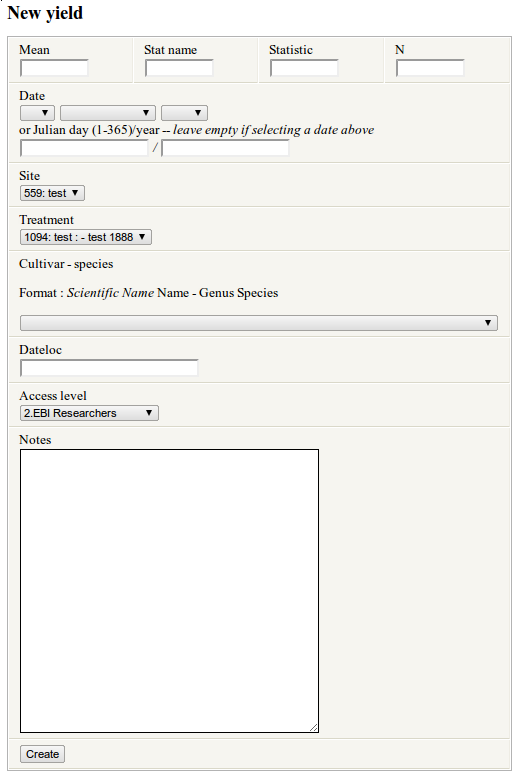
\includegraphics[width=3in]{figures/yields_new.png} 
\caption{Form used to enter a new Yield.}
\label{fig:yields_new}
\end{figure}

\subsection{Adding a PFT}
Plant functional types (PFTs) are used to group plants for statistical modeling and analysis.
PFTs are associated with both a specific set of priors, and a the subset species for which the traits and yields data will be queried.
In many cases, it is appropriate to use default PFTs (e.g. \verb+tempdecid+ is temperate deciduous trees)

In other cases, it is necessary to define pfts for a specific project.
For example, to query a specific set of priors or subset of species, a new PFT may be defined. 
For example, Xiaohui Feng defined PFT's for the species found at the EBI Farm parairie.
Such project-specific PFTs can be defined as \verb+`projectname`.`pft`+ (i.e. \verb+ebifarm.c4grass+ instead of \verb+c4grass+).

\subsection{Adding a Species} \label{sec:addspecies}

 Species that are found or cultivated in the United States should be in the Plants table. 
 Look it up there first.

\subsection{Adding a Cultivar}\label{sec:addcultivar}
\section{BETYdb: Bulk data upload}

 Currently the web interface does not support bulk data upload, although this is a planned feature for BETY 2.0.
 
 For bulk data upload, or for a complete view of the tables in BETY, a blank spreadsheet can be found \href{https://spreadsheets0.google.com/spreadsheet/pub?hl=en&hl=en&key=0Ai_PDCcY5g2JdFN1UDJJdjNsZk9RM0Z6bnFDdlQ0clE&output=html}{online} and can be downloaded in .xls format \href{https://spreadsheets0.google.com/spreadsheet/pub?hl=en&hl=en&key=0Ai_PDCcY5g2JdFN1UDJJdjNsZk9RM0Z6bnFDdlQ0clE&output=xls}{spreadsheet}. 
 Contact \href{mailto:dlebauer@illinois.edu}{David LeBauer} or \href{mailto:mdietze@illinois.edu}{Mike Dietze} for more information about using this method of data upload.

\section{BETYdb: QA/QC with the web interface}
 Quality assurance and quality control (QA/QC) is a critical step that is used to ensure the validity of data in the database and of the analyses that use these data.
 When conducting QA/QC, your data access level needs to be elevated to ``manager''.
 
 \begin{enumerate}
 \item open citation in Mendeley
 \item locate citation in BETYdb
   \begin{itemize}
   \item select 'use'
   \item select 'show'
   \item check that author, year, title, journal, volume, and page information is correct
   \item check that links to URL and PDF are correct, using doi if available
   \item if any information is incorrect, click 'edit' to correct.
   \end{itemize}
 \item check that site(s) at bottom of citation record match site(s) in paper
   \begin{itemize}
   \item check that latitude and longitude are consistent with manuscript, are in decimals not degrees, and have appropriate level of precision \autoref{tab:siteloc}.
   \item click on site name to verify any additional information site information that is present
   \item enter any additional site level information that is found
   \end{itemize}
 \item select  \href{http://ebi-forecast.igb.uiuc.edu/bety/treatments/}{treatments} from menubar
   \begin{itemize}
   \item check that there is a control treatment
   \item ensure that treatment name and definition are consistent with information in the manuscript.
   \item under ``treatments from all citations associated with associated sites'', ensure that there is no redundancy (i.e. if another citations uses the same treatments, it should not be listed separately)
   \item if managements are listed, make sure that managment-treatment associations are correct
   \end{itemize}
 \item check \href{http://ebi-forecast.igb.uiuc.edu/bety/managements/}{managements} if there are any listed on the treatments page.
   \begin{itemize}
   \item if Yield data have been collected, ensure that required managements have been entered
   \item if managements have been entered, ensure that they are associated with the correct treatments
   \end{itemize}
 \item click \href{http://ebi-forecast.igb.uiuc.edu/bety/yields/}{Yields} or \href{http://ebi-forecast.igb.uiuc.edu/bety/traits/}{Traits} to check data.
   \begin{itemize}
   \item check that means, sample size, and statistics have been entered correctly
   \item if data has been transformed, check that transformation was correct in the associated google spreadsheet (or create a new google spreadsheet following instructions in \autoref{sec:googlespreadsheets}).
   \item for any trait data that requires a covariate \autoref{tab:covariates}.
   \end{itemize}

 \end{enumerate}



\section{Acknowledgements}

 Patrick Mulroony pat@life.illinois.edu implemented the data entry interface.
 Moein Azimi, David Bettinardi, and Nick Brady, along with other members of the Dietze lab, have contributed to the ongoing development this document and the web interface that it describes.
 
\section{Appendix}


\subsection{Transformations}

\subsubsection{Statistics}

\begin{table}
  \caption{How to convert statistics from $P$, $LSD$, or $MSD$ to $SE$}
  \label{tab:statconversions}
  \begin{tabular}{llllp{2in}}
    \hline
    from & to & conversion                      & rcode & notes\\ \hline
    P   & SE & $SE = \frac{\bar{X}_1-\bar{X}_2}{t_{1-P/2,2n-2}\sqrt{2/n}}$ &\verb+(x1-x2)/(qt(1-P/2,2*n-2)*sqrt(2/n))+& $\bar{X}_{1,2}$ are two means being compared.      \\
    LSD & SE & $SE = \frac{LSD}{t_{1-\alpha/2,n}*\sqrt{2b}}$ &\verb+LSD/(qt(1-P/2,n)*sqrt(2*b))+ &where $b$ is the number of blocks, $n$ is the number of replicates, and  $n=b$ in a Randomized Complete Block Design \\
    MSD & SE & $SE = \frac{MSD*n}{t_{1-\alpha, 2n-2}*\sqrt{2}}$ & \verb+msd*n/(qt(1-P/2,2*n-2)*sqrt(2))+ \\
    % F, $SS_w$, $df_1$, $df_2$& MSE & &\ref{th:FdfSStoMSE}\\
    \hline
  \end{tabular}
\end{table}

\subsubsection{Variables}
 
\begin{table}
  \caption{Useful conversions for entering site, management, yield, and trait data}
  \label{tab:traitconversion}
  \begin{tabular}{lllp{2in}}
    \hline
    from ($X$) & to ($Y$) & conversion                      & notes\\ \hline
     $X_2=$root production, $X_1=$root biomass & root turnover rate & $Y = X_2/X_1$& \citet{gill2000gpr}\\
    DD$^{\circ}$MM'SS& XX.ZZZZ & $\textrm{XX.ZZZZ} = \textrm{XX} + \textrm{MM}/60+\textrm{SS}/60$& to convert latitude or longitude from degrees, minutes, seconds to  decimal degrees  \\
    lb   & kg & $Y=X\times 2.2$ &      \\
    mm/s   & $\mu$mol CO$_2$ m$^{2}$ s$^{-1}$ & $Y=X\times 0.04$ &       \\
    m$^2$& ha & $Y = X/10^6$&      \\
    g/m$^2$&kg/ha&$Y=X\times 10$ & \\
    US ton/acre &Mg/ha &$Y = X * 2.24$ & \\
    m$^3$/ha&cm& $Y=X/100$& units used for irrigation and rainfall\\
    \% roots &root:shoot (q)& $Y=\frac{X}{1-X}$& $\% \text{roots} = \frac{\text{root biomass}}{\text{total biomass}}$ \\
    $\mu$ mol cm$^{-2}$ s$^{-1}$ & mmol m$^{-2}$s$^{-1}$ & $Y = X/10$& \\
    mol m$^{-2}$ s$^{-1}$& mmol m$^{-2}$s$^{-1}$ & $Y = X/10^6$& \\
    mol  m$^{-2}$ s$^{-1}$&$\mu$mol cm$^{-2}$s$^{-1}$& $Y = X/ 10^5$& \\
    mm s$^{-2}$&mmol m$^{-3}$ s$^{-1}$ &$Y=X/41$ &\citet{korner1988gsc} \\
    mg CO$_2$ g$^{-1}$ h$^{-1}$ & $\mu$mol kg$^{-1}$ s$^{-1}$& $Y = X\times 6.31$& used for root\_respiration\_rate\\
    $\mu$mol&mol& $Y= X\times 10^6$&\\
    julian day (1--365) & date & see \href{http://disc.gsfc.nasa.gov/julian_calendar.shtml}{NASA Julian Calendar}\\
    spacing (m) & density (plants m$^{2}$) &$Y=\frac{1}{\textrm{row spacing}\times\textrm{plant spacing}}$ & \\ 
    kg ha$^{-1}$y$^{-1}$& Mg ha$^{-1}$y$^{-1}$ & $Y= X/1000$& \\
    g m$^{-2}$y$^{-1}$& Mg ha$^{-1}$y$^{-1}$ &$Y= X/100$& \\
    kg & mg & $Y=X\times 10^6$ & \\
    cm$^2$ &m$^2$ &$Y=X\times 10^4$ & \\
    \hline
  \end{tabular}
\end{table}

\subsection{Calculations used in transformations}

\section{Converting from $\frac{\mu\mathrm{L}\ \mathrm{O}_2}{10\mathrm{mg}\ \mathrm{h}}$ to  $\frac{\mathrm{nmol CO}_2}{\mathrm{g}\ \mathrm{s}}$ and $\frac{\mu\mathrm{mol}\ \mathrm{CO}_2}{\mathrm{kg}\ \mathrm{s}}$, including adjustment for temperature}
\label{app:rootrespcalc}

\subsection{Objective:} Convert from root respiration data reported in George et al (where O$_2$ was measured in $\mu$L to units of mass.

In the appendix table, George 2003 reports the range of root respiration rates, converted to $15\ ^\circ C$ and standard units:

$$[11.26, 22.52]  \frac{\mathrm{nmol CO}_2}{\mathrm{g}\ \mathrm{s}}$$


In the original publication Allen (1969), root respiration was measured at  $27\ ^\circ $C. 
The values can be found in table 3 and figure 2. 
The data include a minimum (Group 2 Brunswick, NJ plants) and a maximum (Group 3 Newbery, South Carolina), which I assume are the ones used by George 2003:

$$[27.2, 56.2] \frac{\mu\mathrm{L}\ \mathrm{O}_2}{10\mathrm{mg}\ \mathrm{h}}$$

\subsection{Step 1}
Transformed George 2003 measurements back to the measurement temperature using a rearrangement of equation 1 from George, the standardized temperature of  $15\ ^\circ $C stated in the Georgeh table legend, and  Q$_{10} = 2.075$ from George 2003, and the measurement temperature of $27\ ^\circ $C reported by Allen 1969: 

$$R_T = R_{15}[\exp(\ln(Q_{10})(T- 15))/10]$$

$$[11.26, 22.52] * exp(log(2.075)*(27 - 15)/10)$$

Now we have the values that we would have expected to find in the Allen paper, except that the units need to be converted back to the original:  

$$[27.03,54.07] \mathrm{nmol CO}_2\ \mathrm{g}^{-1}\mathrm{s}^{-1}$$ 

\subsection{Step 2 converting the units}


\subsection{Required constants:}
\begin{itemize}
\item $1\ \mathrm{mol}\ \mathrm{O}_2 = 1\ \mathrm{mol}\ \mathrm{CO}_2$ since respiration is
  $\mathrm{CH}_2\mathrm{O} + \mathrm{O}_2 \to \mathrm{CO}_2 + \mathrm{H}_2\mathrm{O}$
\item density of $\mathrm{O}_2$ at $27^\circ C$: $\frac{7.69 \times 10^5\ \mathrm{ml}\ \mathrm{O}_2}{\mathrm{g}\ \mathrm{O}_2}$ first assume that Allen converted to sea level pressure (101 kPa), although  maybe they were measured at elevation (Allen may have worked at \~{} 900 kPa near Brevard, NC)
\item molar mass of $\mathrm{O}_2$: $\frac{32\mathrm{g}\ \mathrm{O}_2}{\mathrm{mol}}$
\item treat 10mg, which is in the unit of root mass used by Allen, as a unit of measurement for simplicity 
\end{itemize}

Now convert $$[27.03,54.07] \mathrm{nmol CO}_2\ \mathrm{g}^{-1}\mathrm{s}^{-1}$$ to units of $\frac{\mu\mathrm{L}\ \textrm{O}_2}{10\mathrm{mg}\ \mathrm{root}\ \mathrm{h}}$.
The expected result is the original values reported by Allen: $[27.2, 56.2] \frac{\mu\mathrm{L}\ \mathrm{O}_2}{10\mathrm{mg}\ \mathrm{h}}$

$$[27.03, 54.07]\ \frac{\mathrm{nmol}\ \mathrm{CO}_2}{\mathrm{g}\ \mathrm{root}\ \mathrm{s}} \times \frac{1\ \mathrm{g}}{100\times10\mathrm{mg}} \times \frac{3600\ \mathrm{s}}{\mathrm{h}} \times \frac{\mathrm{nmol}\ \mathrm{O}_2}{\mathrm{nmol}\ \mathrm{CO}_2}\frac{3.2 \times 10^{-8}\ \mathrm{g}\ \mathrm{O}_2}{\mathrm{nmol}\ \mathrm{O}_2}\times \frac{7.69\times10^5\ \mu\mathrm{L}\ \mathrm{O}_2}{\mathrm{g}\ \mathrm{O}_2}$$

The result is: 

$$[23.8, 47.8]  \frac{\mu\mathrm{L}\ \textrm{O}_2}{10\mathrm{mg}\ \mathrm{root}\ \mathrm{h}}$$

These are the units reported in the Allen paper, but they appear to be off by the temperature conversion factor, $exp(log(2.075)*(27 - 15)/10)=2.4$, e.g. $[11.9, 23.9]\times 2.4= [28.6,57.4]$, values which are only 5 and 2 percent larger than the original values of $[27.2, 56.2]$, respectively to be acceptable, but not exact. Since the ratio of observed:expected values are different, it is not likely that Q$_{10}$ or the atmospheric pressure at time of measurement would explain this error.  

\subsection{convert to units in BETYdb, find $\textrm{k}$}:


$$\textrm{k}\times\frac{\mu\mathrm{L}\ \textrm{O}_2}{10\mathrm{mg}\ \mathrm{root}\ \mathrm{h}} = \frac{\mu\mathrm{mol}\ \mathrm{CO}_2}{\mathrm{kg}\ \mathrm{s}}$$


$$k =  \frac{\mathrm{g}\ \mathrm{O}_2}{7.69\times10^5\ \mu\mathrm{L}\ \mathrm{O}_2}\times\frac{\mu\mathrm{mol}\ \mathrm{O}_2}{3.2 \times 10^{-5}\ \mathrm{g}\ \mathrm{O}_2} \times \frac{10^5\ \times 10\mathrm{mg}}{\mathrm{kg}} \times \frac{\mathrm{h}}{3600\ \mathrm{s}}= $$ 
$$= 1.13$$



\section{Calculating  $MSE$ given $F$, $df_{\text{group}}$, and $SS$}

Given:
\begin{equation}\label{eq:f}
  F = MS_g/MS_e
\end{equation}


Where $g$ indicates the group, or treatment. 
Rearranging this equation gives:
$$MS_e=MS_g/F$$

Given

$$MS_x = SS_x/df_x$$

Substitute $MS_e/df_e$ for $SS_e$ in the first equation

$$F=\frac{SS_g/df_g}{MS_e}$$

Then solve for $MS_e$

\begin{equation}\label{eq:mse}
  MS_e = \frac{SS_g}{df_g\times F}
\end{equation}

\begin{equation}\label{eq:dft}
  df_{\text{total}}=(df_a+1)\times(df_b+1)...\times(n)-1
\end{equation}
which depends on the experimental design:

for factors a, b... (usually 1 or 2, sometimes 3) where $n$ is the number of replicates within each treatment combination.

\begin{itemize}
\item  one-way anova $df_{\text{total}}=an-1$; where $a$ is the number of treatments 
\item two-way anova without replication $df_{\text{total}}=(a+1)(b+1)-1$ also known as ''randomized complete block design'' (RCBD)
\item two-way anova with $n$ replicates $df_{\text{total}}=(a+1)(b+1)(n)-1$ aka ''RCBD with replication''
\end{itemize}

\subsection{Example}

An example application of this is in \cite{starr2008pra} table 3 (\autoref{fig:starr2008}).  

\begin{figure}
  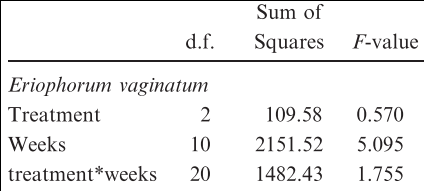
\includegraphics[width=3in]{starr2008.png}
  \caption{Table used to calculate SE from F, from \cite{starr2008pra}.} 
  \label{fig:starr2008}
\end{figure}

The results are from one (two?) factor ANOVA with repeated measures, with treatment and week as the factors and no replication.

We will calculate MSE from the $SS_{\text{treatment}}$ $df_{\text{treatment}}$, and $F$-value given in the table; these are $109.58$, $2$, and $0.570$, respectively; $df_{\text{weeks}}$ is given as $10$.

For the 1997 \textit{Eriphorium vaginatum}, the mean $A_{max}$ in table 4 is $13.49$.

Calculate $MS_e$: 

$$MS_e = \frac{109.58}{0.57 \times 2} = 96.12$$

\section{Bibliography}
\bibliographystyle{plainnat}
\bibliography{bety_documentation_refs}


\end{document}
